\textbf{/F80/} \\
\textbf{Prozess:} Gruppe löschen \\
\textbf{Ziel:} Löschen einer eigenen Gruppe \\
\textbf{Kategorie:} primär \\
\textbf{Vorbedingung:} Erstellung einer Gruppe \\
\textbf{Nachbedingung (Erfolg):} Gruppe ist gelöscht\\
\textbf{Nachbedingung (Fehlschlag):} Gruppe bleibt erhalten\\
\textbf{Akteure:} Administrator der Gruppe \\
\textbf{Auslösendes Ereignis:} Administrator will Gruppe löschen\\
\textbf{Beschreibung:} \\
1. Der Admin geht in das Gruppenmenü
2. Der Admin wählt eine seiner erstellten Gruppen aus \\
3. Der Admin ruft das Menü der Gruppe auf \\
4. Durch wählen der Option "Gruppe löschen" wird die Gruppe gelöscht \\
\textbf{Erweiterung:} \\
\textbf{Alternativen:} \\

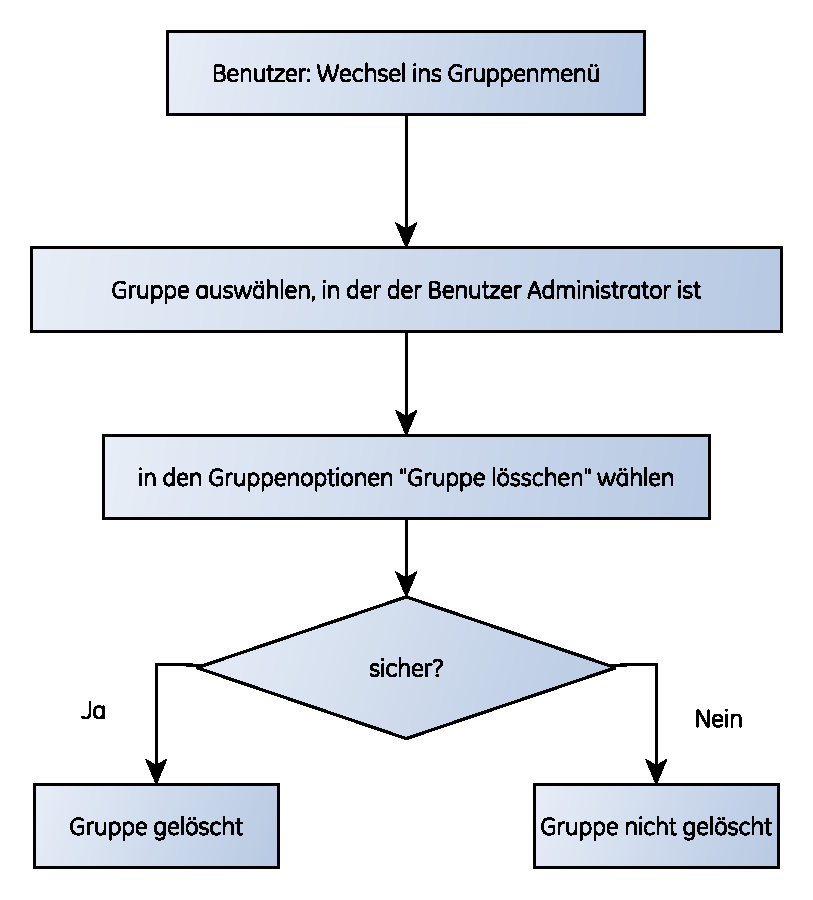
\includegraphics[scale=0.8]{./res/F80_gruppe_loeschen_flowgraph.pdf}
